%%%%%%%%%%%%%%%%%%%%%%%%%%%%%%%%%%%%%%%%%%%%%%%%%%%%%%%%%%%%%%%%%%%%
%%  The file contains the LaTeX shell for BIRS workshop reports.
%%
%%  The reports are being compiled into one volume so you must stick
%%  to the following.
%%
%%  Do not change/add anything before \begin{document}.
%%
%%  There is a list of packages you can uncomment and use.  
%%
%%  The use of TeX/LaTeX macros is NOT permitted.  Reports with macros
%%  will not be accepted. 
%%
%%  Please let LaTeX handle the numbering of your sections, equations, 
%%  figures and tables.
%%
%%  Do not be too concerned about page breaks etc.  These may change
%%  when your document is put into the volume.  We will make sure the
%%  page breaks look okay.
%%
%%  Please use thebibliography environment to do your references.  Use
%%  the format shown in the examples below.
%%
%%  Please use the \includegraphics for including images.  If you
%%  wish, graphics can be sent separately with comments in the tex
%%  file to indicate where they should be included and how big they
%%  they should be.
%%
%%  You can find all of the reports for the BIRS workshops online
%%  under the Publications link.  Select "BIRS 2003 Proceedings" to
%%  view all the reports.  The Scientific Director recommends the
%%  following reports as 'good' examples: Chapters 2, 6, 7, 9, 14, 15
%%  and 22.
%%
%%  Last revised on 24 March 2006.
%%%%%%%%%%%%%%%%%%%%%%%%%%%%%%%%%%%%%%%%%%%%%%%%%%%%%%%%%%%%%%%%%%%%%
\documentclass[10pt]{article}

\setlength{\textwidth}{6.0in}
\setlength{\textheight}{9in}
\setlength{\oddsidemargin}{0.5in}
\setlength{\evensidemargin}{0in}
\setlength{\topmargin}{-0.25in}
\pagestyle{myheadings}

\bibliographystyle{plain}

\usepackage{times}

%%  Please uncomment any package you need to use.
%% 
%%  If you need to use any additional packages please email BIRS
%%   Programme Coordinator, birs@birs.ca, first.
%% 
\usepackage{epsfig}
%% 
%%  \usepackage{amssymb}
%% 
\usepackage{amsmath}
%% 
%%  \usepackage{amsthm}
%% 
\usepackage{graphics}
%% 

\begin{document}

\title{INSERT TITLE OF YOUR WORKSHOP HERE}
\author{INSERT LIST OF ORGANIZERS HERE in the format: name1
(affiliation1),\\ name2 (affiliation2),$\dots$}
\date{INSERT Start Date--End Date HERE}
\maketitle
\vspace{1in}  % This space is so the page break is approximately the
              % same as in the volume.

Start writing here!\\

Here are some suggestions for topics for your sections:

\section{Overview of the Field}

\subsection{Gaussian process}

From a simplified (and likely eroneous?) point of view, a (finite-$\mathrm{N}$-dimensional projection) of a Gaussian process $f_\mathrm{N}$ is defined as:
$$f_\mathrm{N} \sim \text{multinormal}(\mathrm{m}, \mathrm{K})$$
with a certain mean function $\mathrm{m}$ and a covariance matrix $\mathrm{K}$.  
In particular, the elements of $\mathrm{K}$ are defined by a covariance function.   
In our case (and in most Gaussian process applications), we use an \emph{exponentiated quadratic} function:  
$$\forall i,j  \in [\![1,\mathrm{N}]\!] \hspace{1cm} \mathrm{k}_{i,j} = {\gamma^2} \exp\left(-\frac{1}{2}\left(\frac{\lvert x_j-x_i \rvert }{\rho}\right)^2\right)$$
This covariance function capture the "link" between observations along a continuous variable, such as time or space.   
The function is characterized by two parameters: 
\begin{itemize}
    \item a marginal deviation $\gamma$, which controls the variability around the mean (the intensity?)  
    \item a length scale $\rho$, which controls how long/far the correlations persist 
\end{itemize}

\subsection{Application to tree growth}

Now, let's say that we have ringwidth measurements $r_w$ for one tree, for each year $x_n$.
Using one Gaussian process, a simple model would look like this:

$$\forall x_n  \hspace{0.5cm} \log{r_w(x_n)} \sim \text{normal}(\mu + f(x_n), \sigma^2)$$
with:
$$\vec{f} \sim \text{multinormal}(\vec{0}, \mathrm{K})$$
The two equations are equivalent to:

$$\log\vec{{\text{rw}}} \sim \text{multinormal}(\vec{\mu}, \hspace{0.08cm} \Sigma + \mathrm{K})$$
where:

$$
    \vec{\mu} = \begin{bmatrix}
               \mu \\
               \mu \\
               \vdots \\
               \mu
    \end{bmatrix}
    \hspace{1cm}
	\Sigma = 
	\begin{bmatrix}
		\sigma^2  & 0 & \ldots & 0 \\
		0 & \ \sigma^2  & \ldots  & \vdots\\
		\vdots & \vdots & \ddots & \vdots \\
		0 & \ldots &  \ldots & \sigma^2 
	\end{bmatrix}
$$

\noindent In practice, we choose to model the $\log$ of ringwidth with two Gaussian processes:  
\begin{itemize}
    \item one \textbf{long-term scale} Gaussian process $f_{\text{long}}$, to capture the long-term variation of tree growth, likely related to allometric constraints   
    \item one \textbf{short-term scale} Gaussian process $f_{\text{short,p}}$ per stand $p$, to capture some climatic variations over several years
\end{itemize}

\noindent The long-term scale GP is characterized by one pair of parameters $\{\gamma_{\text{sp}}, \rho_{\text{sp}}\}$ per species $sp$. The short-term scale GP is characterized by two parameters $\{\gamma_{\text{short}}, \rho_{\text{short}}\}$, common across all stands. The short-term scale does not depend on species, but its effect is scaled by a factor $\kappa_\text{sp}$ (see below). We chose two different prior models for these two Gaussian processes, to have the prior mass of $\rho_{\text{short}}$ between 3 and 10 years, and the prior mass of $\rho_{\text{sp}}$ between 20 and 60 years.

\vspace{0.5cm}

\noindent The full model is, for $n$ observations for one tree $k$ of the species $sp$ on the stand $p$:

$$\log\vec{\text{rw}}_{sp,p,k} \sim \text{multinormal}(\vec{\mu_{sp,p}}, \hspace{0.08cm} \Sigma + \mathrm{K_{sp}})$$
with:
$$
\log\vec{\text{rw}}_{sp,k} = 
\log \circ \begin{bmatrix}
  \text{rw}_{sp,p,k}(t_1) \\
  \text{rw}_{sp,p,k}(t_2) \\
  \vdots \\
  \text{rw}_{sp,k}(t_n)
\end{bmatrix}
\hspace{1cm}
\log\vec{\mu}_{sp,p} = 
\log \circ \begin{bmatrix}
  \mu_{sp,p}(t_1) \\
  \mu_{sp,p}(t_2) \\
  \vdots \\
  \mu_{sp,p}(t_n)
\end{bmatrix}
$$

$$ \forall i  \in [\![1,\mathrm{n}]\!]  \hspace{0.5cm} \mu_{sp,p}(t_i)= \alpha
    + \beta_{\text{GSL}} * \text{GSL}(p,t_i)
    + \beta_{\text{GDD}}  * \text{GDD}(p,t_i)
    + \beta_{\text{SM}}  * \text{SM}(p,t_i)
    + \kappa_{\text{sp}}
    * f_{\text{short,p}}(t_i)$$

$$\vec{f}_{\text{short,p}} \sim \text{multinormal}(\vec{0}, \mathrm{K_\text{short}})$$

\noindent We look at three different climate predictors, at the stand scale:
\begin{itemize}
    \item the growing season length $\text{GSL}(p,t_i)$, in days
    \item the growing degree days $\text{GDD}(p,t_i)$ accumulated during the growing season, in $\text{x}10$ $^{\circ}$C
    \item the mean soil moisture $\text{SM}(p,t_i)$ (weighted average across soil horizons) during the growing season, in $\%$
\end{itemize}

\section{Recent Developments and Open Problems}

\subsection{Study area}

\begin{figure}[h]
    
\includegraphics[width = 5cm]{figures/sites.png}
\end{figure}

\clearpage

\subsection{Retrodictive check}

We can examine how the model fit some trees in one particular stand:

\begin{figure}[h]
    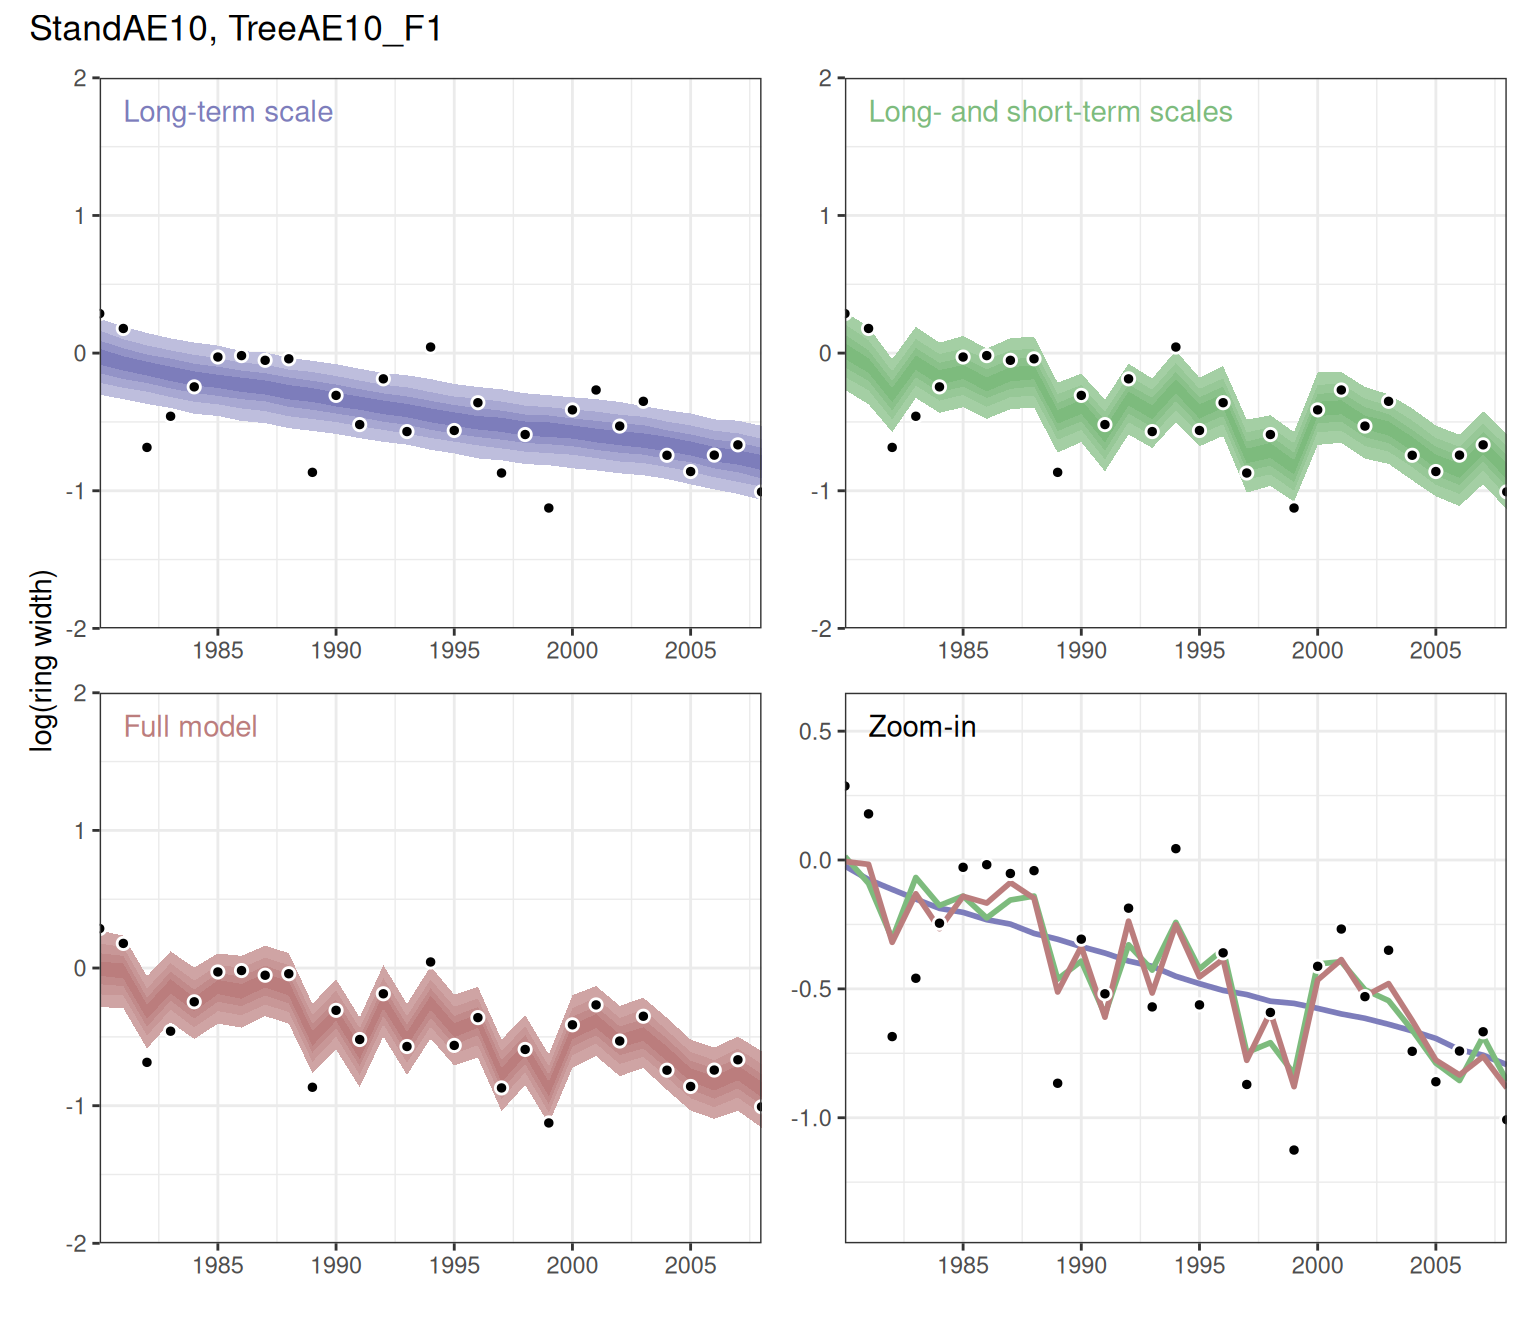
\includegraphics[width = 12cm]{figures/standae10_treef1.png}
\end{figure}

\begin{figure}[h]
    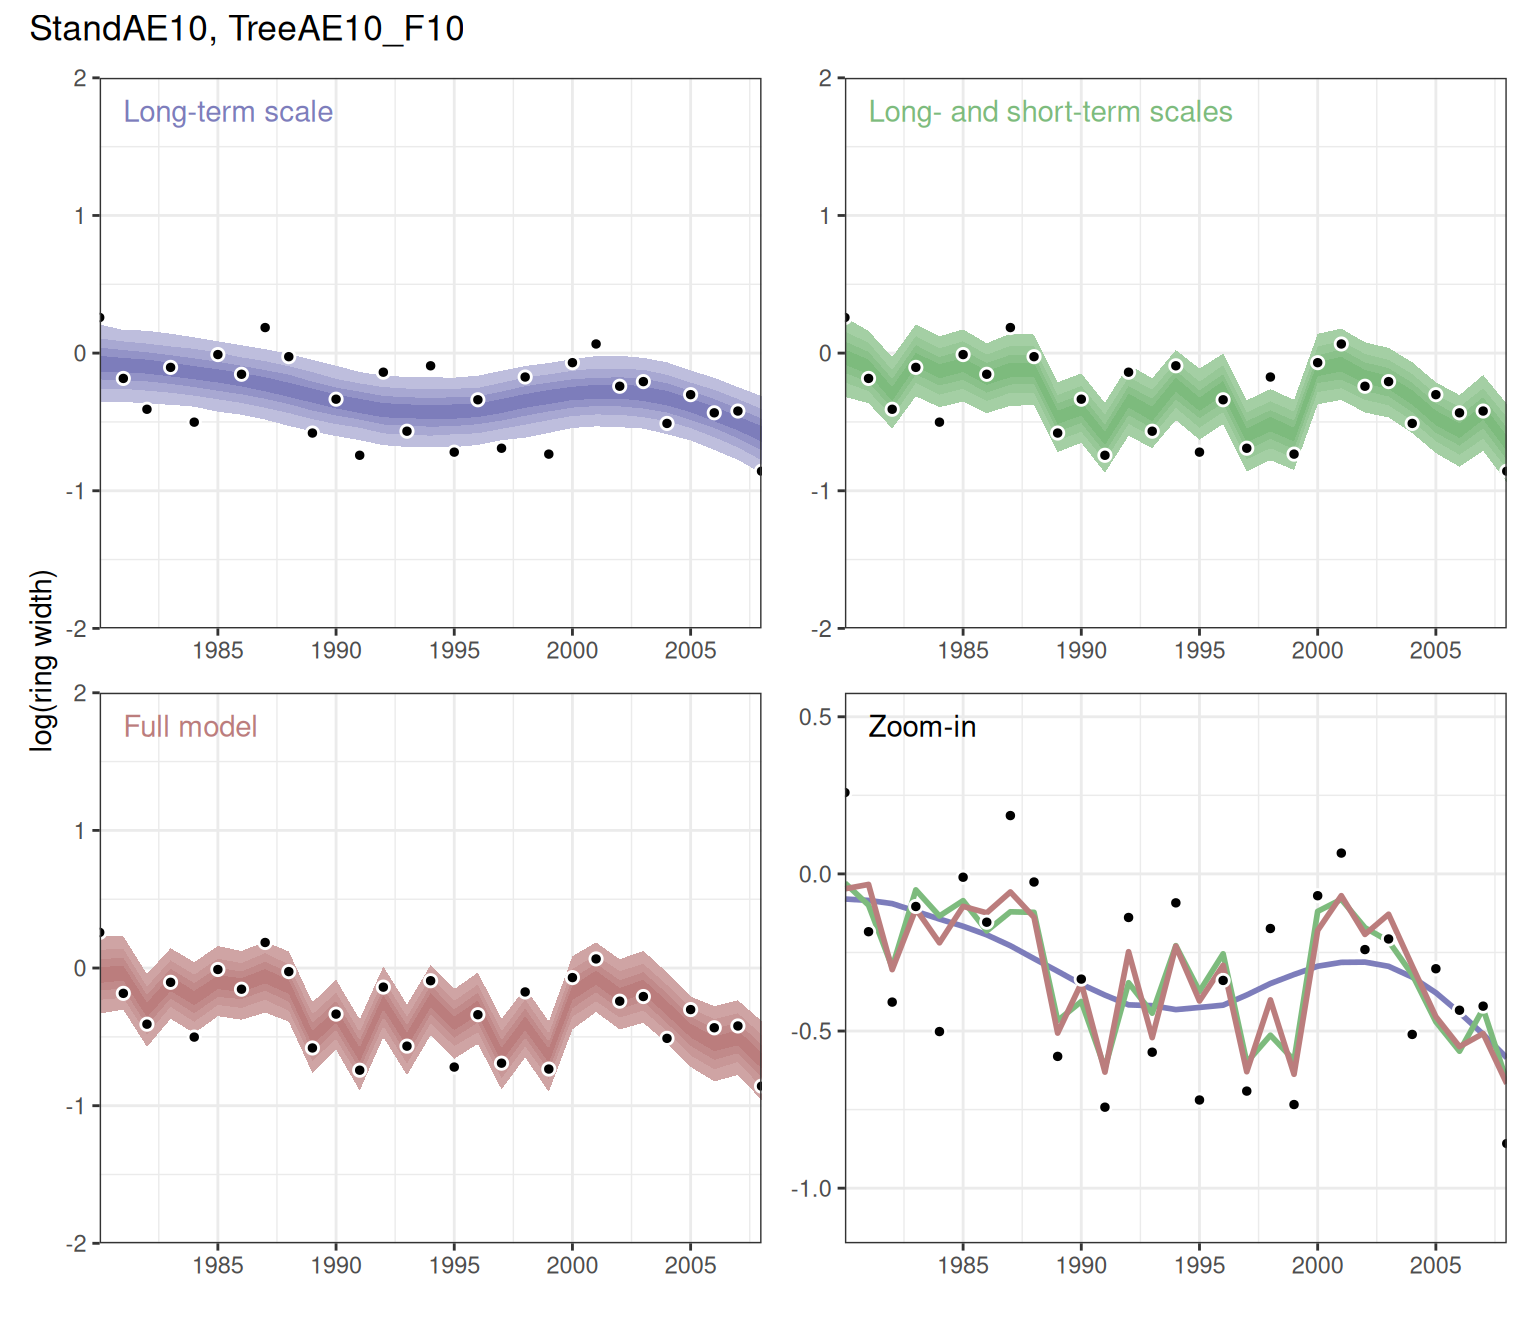
\includegraphics[width = 12cm]{figures/standae10_treef10.png}
\end{figure}

\begin{figure}[h]
    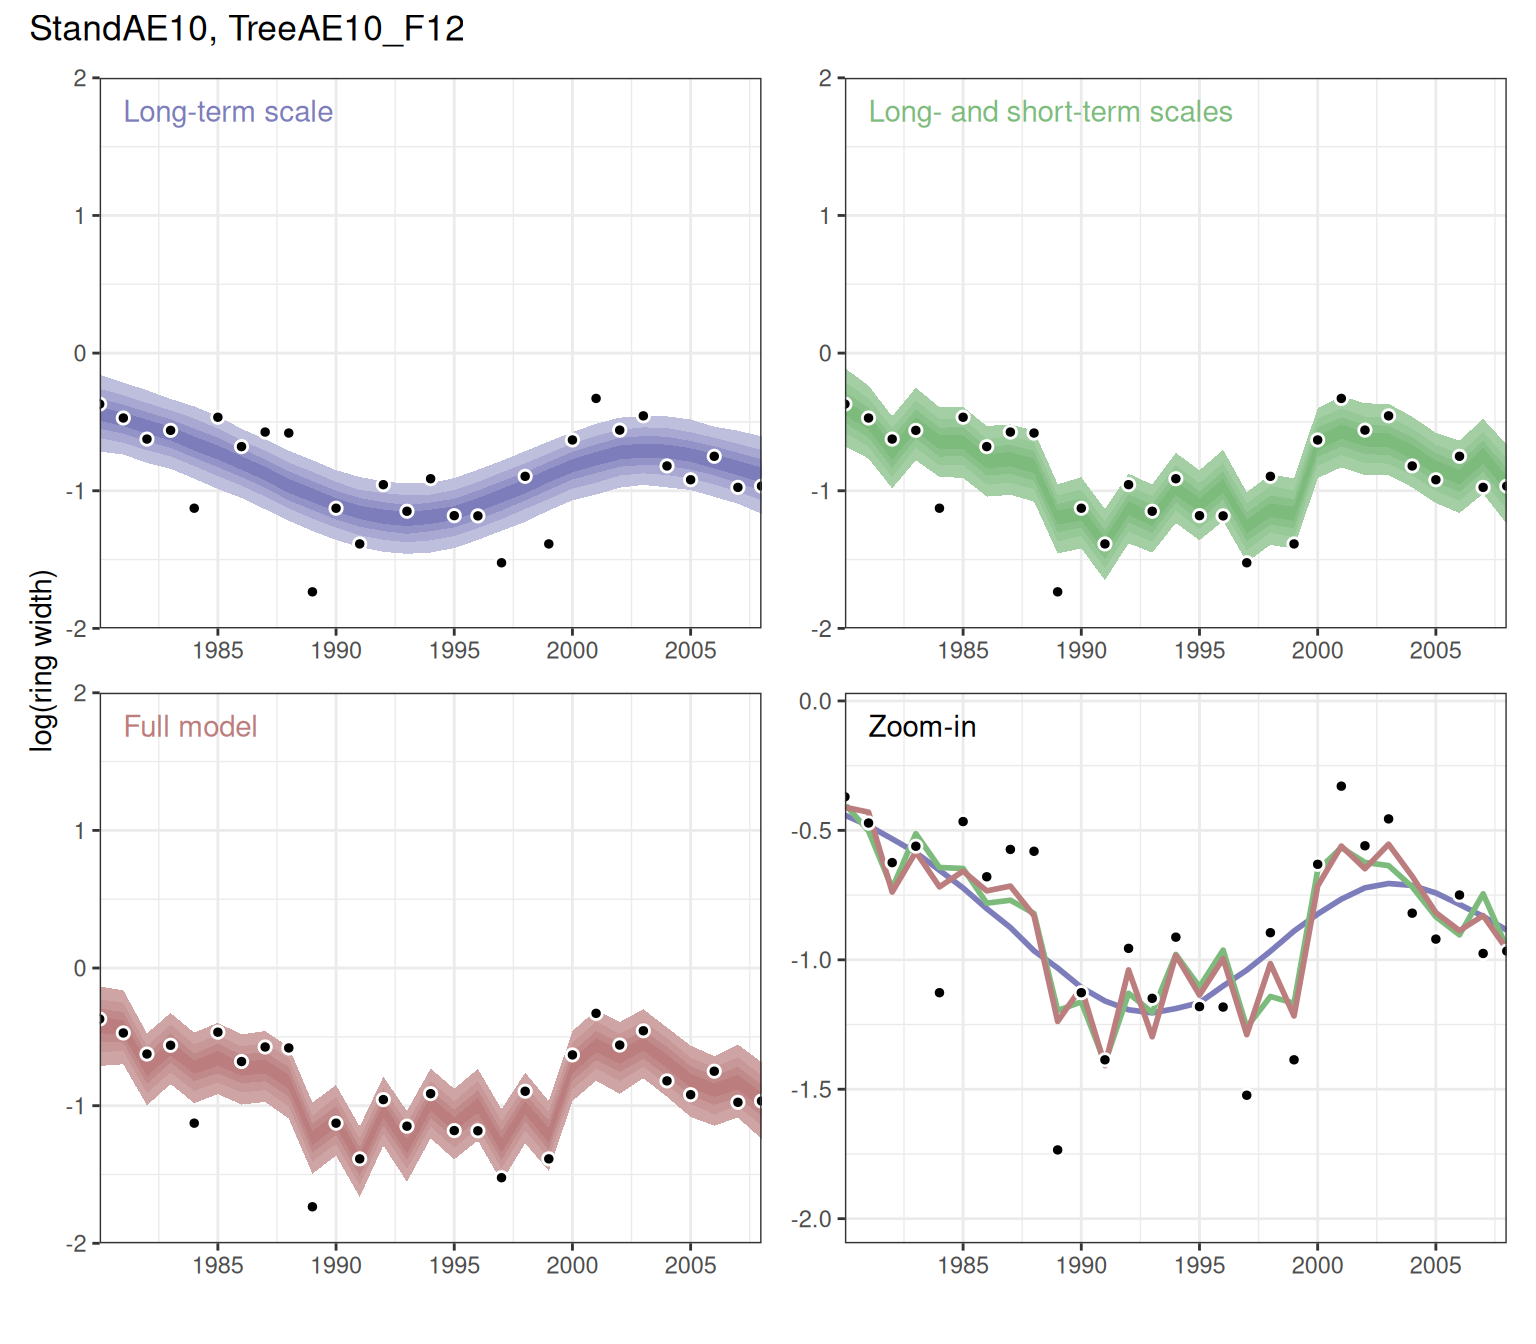
\includegraphics[width = 12cm]{figures/standae10_treef12.png}
\end{figure}

\clearpage

\section{Presentation Highlights}

\section{Scientific Progress Made}

\section{Outcome of the Meeting}


\end{document}

